\documentclass[10pt,letterpaper]{article}
\usepackage[letterpaper, margin=0.5in]{geometry}
\usepackage{tikz}
\usepackage{ifthen}

\begin{document}

\par\noindent
Goal:\break
\includegraphics[width=0.5\linewidth]{reference_images/abs_graph.png}

\par\noindent
TikZ:\break
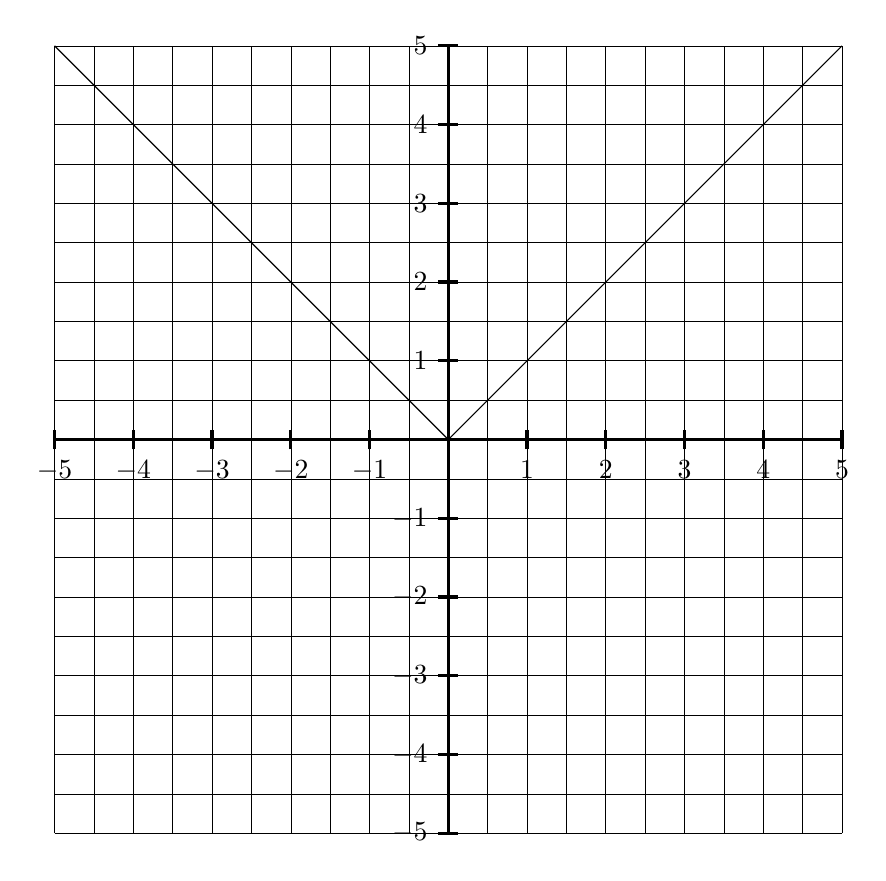
\begin{tikzpicture}
	% Coordinate axes
	\draw[very thick] (-5,0) -- (5,0);
	\draw[very thick] (0,-5) -- (0,5);

	% Coordinate grid
	\draw[step=0.5, very thin] (-5,-5) grid (5,5);

	% Draw the function
	\draw (-5,5) -- (0,0) -- (5,5);

	% Stylize coordinate axes
	\foreach \x in {-5,...,5} {
		\draw[very thick] (\x,-0.125) node[anchor=north]{$\ifthenelse{\x=0}{}{\x}$} -- (\x,0.125);
		\draw[very thick] (-0.125,\x) node[anchor=east]{$\ifthenelse{\x=0}{}{\x}$} -- (0.125,\x);
	}
\end{tikzpicture}

\end{document}